%%%%%%%%%%%%%%%%%%%%%%%%%%%%%%%%%%%%%%%%%%%%%%%%%%%%%%%%%%%%%%%%%%%%%%%%%%%%%%%%%%%%%
% PACOTES                                                                           %
%%%%%%%%%%%%%%%%%%%%%%%%%%%%%%%%%%%%%%%%%%%%%%%%%%%%%%%%%%%%%%%%%%%%%%%%%%%%%%%%%%%%%
\documentclass[a4paper,12pt]{article}

%-----------------------------------------------------------------------------------%
% LAYOUT DA PÁGINA                                                                  %
%-----------------------------------------------------------------------------------%
\usepackage[top=2.5cm, bottom=2.5cm, left=2.5cm, right=2.5cm]{geometry}

%-----------------------------------------------------------------------------------%
% FORMATAÇÃO DO TEXTO                                                               %
%-----------------------------------------------------------------------------------%
\usepackage{setspace} % Permite definir o espaçamento entre linhas

%-----------------------------------------------------------------------------------%
% PACOTES DE IMAGENS                                                                %
%-----------------------------------------------------------------------------------%
\usepackage[pdftex]{graphicx}
\pdfsuppresswarningpagegroup=1 % A warning issued when several PDF images are
% imported in the same page. Mostly harmless, can be almost always supressed.
%\usepackage[pstarrows]{pict2e} % Amplia as funcionalidades do ambiente picture
\usepackage{tikz}
\usetikzlibrary{shapes, arrows, arrows.meta, angles, quotes}

%-----------------------------------------------------------------------------------%
% PACOTES DE TABELAS                                                                %
%-----------------------------------------------------------------------------------%
\usepackage{array} % Facilita a formatação de tabelas
\usepackage{longtable} % Permite criar tabelas que quebram de página

%-----------------------------------------------------------------------------------%
% PACOTES DE CODIFICAÇÃO DE FONTES                                                  %
%-----------------------------------------------------------------------------------%
\usepackage[utf8]{inputenc} % Permite o uso de caracteres ISO 8859-1, incluindo os
%                               caracteres acentuados diretamente.
\usepackage[T1]{fontenc} % Uso de fontes T1, necessário para tratar caracteres
%                          acentuados como um único bloco.

%-----------------------------------------------------------------------------------%
% PACOTES DE LÍNGUAS                                                                %
%-----------------------------------------------------------------------------------%
\usepackage[french]{babel} % Seleciona a língua do documento, definindo nomes de
%                              seções, nome do índice, da bibliografia, etc. Em caso
%                              de documento com mais de uma língua, a padrão é a
%                              última.
\NoAutoSpaceBeforeFDP % Utilizar em francês se quiser evitar espaços antes de :

%-----------------------------------------------------------------------------------%
% PACOTES DE FONTES                                                                 %
%-----------------------------------------------------------------------------------%
% KP Serif                                                                          %
% - - - - - - - - - - - - - - - - - - - - - - - - - - - - - - - - - - - - - - - - - %
\usepackage{kpfonts}

%-----------------------------------------------------------------------------------%
% PACOTES DIVERSOS                                                                  %
%-----------------------------------------------------------------------------------%
\usepackage{icomma} % Permite uso de vírgula como separador decimal
\usepackage{url} % Pacote para não ter problemas com URLs. Usar \url{}
\usepackage[hidelinks]{hyperref}

%%%%%%%%%%%%%%%%%%%%%%%%%%%%%%%%%%%%%%%%%%%%%%%%%%%%%%%%%%%%%%%%%%%%%%%%%%%%%%%%%%%%%
% CONFIGURAÇÕES                                                                     %
%%%%%%%%%%%%%%%%%%%%%%%%%%%%%%%%%%%%%%%%%%%%%%%%%%%%%%%%%%%%%%%%%%%%%%%%%%%%%%%%%%%%%

%-----------------------------------------------------------------------------------%
% FORMATAÇÃO DO TEXTO                                                               %
%-----------------------------------------------------------------------------------%
%\onehalfspacing % Espaçamento 1 1/2 (definido no pacote setspace)
\setstretch{1.1}
\setlength{\parskip}{6pt plus 2pt minus 1pt}

\renewcommand{\floatpagefraction}{0.99}
\renewcommand{\topfraction}{0.99}
\renewcommand{\bottomfraction}{0.99}
\renewcommand{\textfraction}{0.01}

%%%%%%%%%%%%%%%%%%%%%%%%%%%%%%%%%%%%%%%%%%%%%%%%%%%%%%%%%%%%%%%%%%%%%%%%%%%%%%%%%%%%%
% ESTRUTURA DO DOCUMENTO                                                            %
%%%%%%%%%%%%%%%%%%%%%%%%%%%%%%%%%%%%%%%%%%%%%%%%%%%%%%%%%%%%%%%%%%%%%%%%%%%%%%%%%%%%%
\begin{document}

\title{2I013 Projet \\ Groupe 1 : Football et stratégie}
\author{Ariana Carnielli et Parth Shah}
\date{}

\maketitle
\thispagestyle{empty}
\pagenumbering{Alph}

\tableofcontents
\newpage

\pagestyle{plain}
\pagenumbering{arabic}

\section{Introduction}

Ce projet s’intéresse à la programmation des stratégies pour l’automatisation des joueurs dans le jeu de  « football » SoccerSimulator (disponible sur \url{https://github.com/baskiotisn/SoccerSimulator-2017}). Il s'agit d'un jeu codé en Python où les joueurs peuvent s’affronter dans plusieurs types de matchs : en 1 contre 1, en 2 contre 2 ou encore en 4 contre 4. Les joueurs et la balle peuvent se déplacer partout sur un terrain de jeu dont la taille est fixée par deux constantes et est constitué de deux cages placées aux bords verticaux. Si la balle touche les bords du terrain, elle rebondit, par contre les joueurs ne rebondissent pas et perdent toute leurs vitesses. Les joueurs ne sont pas considérés comme des obstacles à la balle, celle-ci peut les croiser sans rebondir. Chaque match est joué en temps discret, donné aussi par une constante. À chaque pas de temps le jeu actualise la position de chaque objet mobile sur le terrain et vérifie si un but a été marqué. Dans ce cas, les positions des joueurs et de la balle sont réinitialisées. Le jeu se joue de manière autonome, chaque joueur choisissant une action à chaque pas de temps en accord à la stratégie qui lui a été passée.

L’objectif est d’implémenter des stratégies permettant à nos joueurs de gagner la plus grande quantité de matchs contre les stratégies adverses codés par d'autres binômes. Dans ce rapport, nous présenterons la démarche mise au point lors de la conception des stratégies tout en abordant les problèmes rencontrés. Dans un second temps nous exposerons des stratégies que nous avons écrites et l'implémentation de l’algorithme génétique pour leur optimisation ainsi que l’implémentation des arbres de décision. Une conclusion récapitulera les principaux points de ce rapport et les compétences acquises.

\section{Démarche utilisée et problèmes rencontrés}

Pour construire des stratégies, plusieurs classes étaient à notre disposition, notamment \texttt{SoccerAction}, \texttt{Vector2D} et \texttt{SoccerState}. \texttt{Vector2D} contient deux coordonnées \texttt{x} et \texttt{y} ainsi que des méthodes pour, par exemple, calculer la norme d’un vecteur donné et son angle par rapport aux axes des coordonnés. Quant à \texttt{SoccerAction}, celui-ci est composé de deux \texttt{Vector2D} : un qui donne la direction du mouvement du joueur et un autre qui donne la direction du shoot. \texttt{SoccerState} contient toutes les informations nécessaires pour connaitre l’état du jeu à un moment donné y compris la position et la vitesse de la balle et de tous les joueurs. 

Il existe déjà une classe \texttt{Strategy} donnant la base pour la construction d'une stratégie : Toute classe de stratégie que nous avons codé hérite de celle-ci. Une stratégie doit implémenter une méthode \texttt{compute\_strategy} qui prend en argument l'état du jeu à travers un \texttt{SoccerState} et l'identification d'un joueur et retourne un \texttt{SoccerAction} à chaque pas de temps. Au départ nos stratégies étaient des classes indépendantes regroupés dans un fichier appelé \texttt{strategy.py}.
	
Comme nous n’avions aucune expérience sur la conception de stratégies, nous avons tout d’abord essayé de coder une petite stratégie telle qu’un fonceur, en reprenant l’exemple vu en cours, qui court vers la balle et tire au but. Notre intention était de l’utiliser principalement en 1 contre 1. Nous nous sommes rendu compte après quelques essais qu’il serait intéressant de ne pas encombrer la stratégie avec des tests pour voir si le joueur a la balle, etc., car à chaque fois que nous voulions changer un paramètre ou les choix faits par la stratégie, il fallait changer tout le code. Nous avons ainsi créé une classe appelée \texttt{ToolBox} avec des méthodes qui retournaient les résultats des tests fréquents qu’on utilisait, dans un fichier nommé \texttt{toolbox.py}.

Au fur et à mesure du projet nous étions amenés à développer de nombreuses stratégies et nous avons remarqué que plusieurs d'entre elles partageaient des morceaux de code suffisamment complexes pour ne pas être dans \texttt{ToolBox}. Nous avons alors rajouté de couches entre nos stratégies et \texttt{ToolBox} en créant d'autres classes. Cela a permis également de rendre le code plus lisible et modulaire. Nous avons mis au point deux fichiers en plus de \texttt{toolbox.py} : \texttt{action.py} et \texttt{comportement.py}. Ainsi, en cas de problème à l’exécution, nous pouvions le trouver plus facilement et modifier seulement la partie de la fonction ou méthode concernée, plutôt que l’intégralité du code.

Nous avons décidé de laisser \texttt{ToolBox} avec toutes les méthodes retournant des booléens, des \texttt{Vector2D} et des listes de \texttt{Vector2D}. Les fichiers \texttt{action.py} et \texttt{comportement.py} ont chacun une classe homonyme : \texttt{Action} contient des méthodes qui retournent des \texttt{SoccerAction} alors que \texttt{Comportement} utilise les méthodes dans \texttt{ToolBox} et \texttt{Action} pour bien choisir le \texttt{SoccerAction} qu'une stratégie doit retourner à chaque pas de temps. Nous avons choisi de séparer les comportements des stratégies afin d’être capable d’appeler plusieurs comportements dans une stratégie quelconque. À la fin, nous avons trouvé cela un peu redondant car nos stratégies appellent uniquement un comportement même si le fait de séparer stratégie et comportement a été utile dans une stratégie décrite plus en détail dans la section suivant.

Tous nos fichiers ont été mis dans un même module contenant un fichier principal \texttt{\_\_init\_\_.py}, où la fonction de création de joueurs en appelant nos stratégies a été placée. Pour ce faire, nous avons eu besoin de la commande \texttt{import} de Python pour l'utilisation d’une classe ou bien d’une fonction écrite dans un autre fichier. Au début, lorsque nous lancions notre fichier exécutable, quelques erreurs apparaissaient à cause des \texttt{import} non aboutis. En effet, la syntaxe de \texttt{import} en Python change selon la version du langage et si l'importation est absolue ou relative. Nous avons donc utilisé exclusivement Python 3, qui utilise des import relatifs explicites, pour régler les soucis.

Nous nous sommes mis à développer également d’autres stratégies plus intéressantes qu’un fonceur, notamment des défenseurs et des dribleurs. Le développement continu de ces stratégies était indispensable pour contrer les améliorations apportées par les autres binômes à leurs stratégies, afin de permettre ainsi une bonne cohésion entre nos joueurs et un équilibre entre la quantité de buts marqués et encaissés pour enfin obtenir un bon rang dans les classements. La section suivante présentera plus en détails nos principales stratégies, leur fonctionnement et les raisonnements derrière nos choix.

Après quelques séances nous nous sommes rendu compte que la meilleure façon de battre tous nos adversaires était d’étudier plus en détail chacune de leurs stratégies et d’en exploiter les faiblesses afin d'avoir l’avantage. C’est pourquoi nous avons commencé à télécharger les modules des autres binômes depuis leurs dossiers en ligne sur \emph{Github}. Pour chaque groupe, nous essayions d’améliorer et de réajuster notre code en fonction des résultats obtenus en simulant des matchs pour enfin arriver à une moyenne de victoires convenable. 

En revanche, il n’était pas toujours facile de trouver une riposte contre les stratégies des autres groupes. Certaines stratégies étaient si bien codées qu’il fallait du temps pour d’abord mettre au point de nouvelles stratégies pour contrer une attaque ou intercepter la balle par exemple, d’autant plus que ces tests devaient être réalisés contre l’ensemble des autres binômes. En outre, certaines étaient mises en ligne quelques instants avant les résultats finaux, nous empêchant ainsi de pouvoir travailler sur les stratégies récentes. En utilisant la recherche exhaustive et l'algorithme génétique nous avons enfin automatisé une partie du processus d’amélioration de nos stratégies, dont la démarche sera présenté dans la Section \ref{4}.

\section{Présentation des stratégies}
\label{3}

Cette section présente les principales \og familles \fg{} de stratégies que nous avons codées à la main pour ce projet : Fonceur, Dribbleur, Défenseur et Attaquant. Cette division suit l'évolution de notre code dans le sens où le Fonceur et ses améliorations ont été les premières stratégies codées, suivies par le Dribleur et le Défenseur qui nous ont permis de passer aux matchs 2 contre 2 et enfin l'Attaquant qui a été crée pour les matchs 4 contre 4.   

\subsection{Fonceur}

Comme nous avons dit précédemment, la première famille de stratégies codée a été le Fonceur qui peut être représenté par l'arbre de décision de la Figure \ref{Figure1}.

\begin{figure}[ht]
\centering
\tikzstyle{block} = [rectangle, rounded corners=3mm, very thick, font=\small, draw=blue!50!white, fill=blue!10!white]
\tikzstyle{decision} = [diamond, rounded corners=3mm, shape aspect=2.5, very thick, font=\small, draw=red!50!white, fill=red!10!white, inner sep=0mm]

\begin{tikzpicture}

\node[decision] (test1) at (0, 0) {\parbox[c][\height][c]{4cm}{\centering Peut tirer? }};
\node[block, anchor = north] (oui) at (-3, -2) {\parbox[c][\height][c]{4cm}{\centering Tirer vers le centre du but}};
\node[block, anchor = north] (non) at (3, -2) {\parbox[c][\height][c]{4cm}{\centering Courir vers le ballon}};
\draw[thick, -Stealth] (test1) -- node[midway, above left]{\small Oui} (oui);
\draw[thick, -Stealth] (test1) -- node[midway, above right]{\small Non} (non);

\end{tikzpicture}
\caption{Arbre de décision du Fonceur}
\label{Figure1}
\end{figure}

Dans un premier temps cette stratégie a été codée sans aucun paramètre mais nous avons ensuite identifié quelques uns ayant une influence sur le comportement et l’efficacité de cette stratégie : l’accélération du joueur quand il court, l'accélération de son tir et la quantité de pas de temps en avance qu'il essaie pour prévoir la position du ballon.

Lorsque ce fonceur joue contre d'autres stratégies de fonceur identiques ou très similaires, il arrive assez souvent qu'on tombe sur une situation de \og blocage \fg, où les deux joueurs courent ensemble vers le ballon, arrivant et tirant au même moment en directions opposées, à laquelle le ballon part dans une direction essentiellement aléatoire et aucun des deux joueurs n'arrive à marquer un but. Ce blocage peut être partiellement résolu en changeant le nombre de pas de temps de prévision de la position du ballon, mais cette solution ne donne pas en général des résultats satisfaisants, surtout car une quantité de pas de temps peut être très bonne pour certaines variantes du fonceur, mais pas pour d'autres. Cela nous a motivés à créer une stratégie plus élaborée, le Dribbleur, décrit dans la prochaine partie.

\subsection{Dribbleur}

La famille de stratégies qui forme la pièce maitresse de notre jeu est le Dribbleur dont l'arbre de décision représentatif est donné sur la Figure \ref{Figure3}. 

\begin{figure}[ht]
\centering
\tikzstyle{block} = [rectangle, rounded corners=3mm, very thick, font=\small, draw=blue!50!white, fill=blue!10!white]
\tikzstyle{decision} = [diamond, rounded corners=3mm, shape aspect=2.5, very thick, font=\small, draw=red!50!white, fill=red!10!white, inner sep=0mm]

\begin{tikzpicture}

\node[decision] (tirer) at (0, 0) {\parbox[c][\height][c]{4cm}{\centering Peut tirer? }};
\node[decision, anchor = north] (tirer_oui) at (-3.5, -0.6) {\parbox[c][\height][c]{4cm}{\centering Très proche de\\ la cage adverse?}};
\node[block, anchor = north] (tirer_non) at (3.5, -1.1) {\parbox[c][\height][c]{3cm}{\centering Courir vers le ballon}};

\draw[thick, -Stealth] (tirer) -- node[midway, above left]{\small Oui} (tirer_oui);
\draw[thick, -Stealth] (tirer) -- node[midway, above right]{\small Non} (tirer_non);

\node[block, anchor = north] (proche_oui) at (-6.2, -3.6) {\parbox[c][\height][c]{3cm}{\centering Tirer vers le centre du but}};
\node[decision, anchor = north] (proche_non) at (0, -3.0) {\parbox[c][\height][c]{4cm}{\centering Il y a un adversaire devant?}};

\draw[thick, -Stealth] (tirer_oui) -- node[midway, above left]{\small Oui} (proche_oui);
\draw[thick, -Stealth] (tirer_oui) -- node[midway, above right]{\small Non} (proche_non);

\draw[thick, -Stealth] (proche_non) -- node[midway, above]{\small Non} (proche_oui);

\node[decision, anchor = north] (ennemi_oui) at (0, -6.0) {\parbox[c][\height][c]{4cm}{\centering L'adversaire peut \\tirer aussi?}};

\draw[thick, -Stealth] (proche_non) -- node[midway, left]{\small Oui} (ennemi_oui);

\node[block, anchor = north] (peut_tirer_oui) at (-4.1, -8.7) {\parbox[c][\height][c]{4cm}{\centering Tirer vers le champ adversaire le plus fort possible}};

\node[decision, anchor = north] (peut_tirer_non) at (4.1, -7.9) {\parbox[c][\height][c]{4cm}{\centering \vspace*{3pt}L'adversaire est dans \\la cage \textbf{et} on est \\proche de la cage?}};


\draw[thick, -Stealth] (ennemi_oui) -- node[midway, above left]{\small Oui} (peut_tirer_oui);
\draw[thick, -Stealth] (ennemi_oui) -- node[midway, above right]{\small Non} (peut_tirer_non);

\node[block, anchor = north] (proche_et_cage_oui) at (1.9, -11.2) {\parbox[c][\height][c]{3cm}{\centering Tirer vers le coin de la cage}};

\node[block, anchor = north] (proche_et_cage_non) at (6.3, -11.2) {\parbox[c][\height][c]{3cm}{\centering \textbf{Dribbler l'adversaire}}};

\draw[thick, -Stealth] (peut_tirer_non) -- node[midway, above left]{\small Oui} (proche_et_cage_oui);
\draw[thick, -Stealth] (peut_tirer_non) -- node[midway, above right]{\small Non} (proche_et_cage_non);


\end{tikzpicture}
\caption{Arbre de décision du Dribbleur}
\label{Figure3}
\end{figure}

En comparant les Figures \ref{Figure1} et \ref{Figure3} on remarque que le Dribbleur a le même comportement que le Fonceur s'il n'a pas le ballon, s'il est très proche de la cage adverse ou s'il n'existe pas d'adversaire devant lui. Cependant il a un comportement plus élaboré dans d'autres situations. Lorsqu'il arrive au ballon au même temps qu'un adversaire, il essaie de contrer le tir adverse en faisant un tir d'accélération maximale vers le champ adverse, sans viser la cage. Dans le cas où l’équipe adverse a un gardien, c'est-à-dire un joueur au voisinage immédiat de la cage, le Dribbleur frappe en visant le coin de la cage le plus proche de lui. Enfin, s'il n'est pas proche de la cage et il existe un joueur adverse devant lui qui n'est pas trop loin, il dribble selon le schéma de la Figure \ref{Figure4}.

\begin{figure}[ht]
\centering
\begin{tikzpicture}
\node[rectangle, thick, draw=red!80!white, fill=red!30!white, minimum size=0.5cm] (me) at (0, 0) {};
\node[rectangle, thick, draw=blue!80!white, fill=blue!30!white, minimum size=0.5cm] (other) at (2, 1) {};

\node[rectangle, thick, draw=black!50!white, fill=black!30!white, minimum width=0.2cm, minimum height=2cm, anchor = east] (goal) at (5, -1) {};

\draw[thick, -Stealth] (me.center) -- (other.center);
\draw[thick, -Stealth] (me.center) -- (goal.center);
\draw (5, -2.5) -- (5, 1.5);
\coordinate (A) at (goal.center);
\coordinate (B) at (me.center);
\coordinate (C) at (other.center);
\draw pic[draw=black, thick, angle radius=0.75cm, "$\theta$", angle eccentricity = 1.5] {angle = A--B--C};
\end{tikzpicture}
\caption{Schéma d'un dribble : Dribbleur en rouge, adversaire en bleu, cage en gris}
\label{Figure4}
\end{figure}

Pour le dribble, le joueur détermine les vecteurs entre lui-même et le centre du but adverse et entre lui-même et le joueur adverse le plus proche devant lui, calculant ensuite l'angle $\theta$ entre ces vecteurs. Si $\theta$ est trop grand, il considère que l'autre joueur ne bloque pas son chemin au but et ne fait pas de dribble. Sinon, il fait un dribble : si l’adversaire est situé en bas par rapport au joueur, il dribble vers le haut, et au contraire si l’adversaire est situé en haut par rapport au joueur, il dribble vers le bas.
 
Un souci observé avec cette implémentation de dribble est que, dans certaines \mbox{situations} où le joueur, son adversaire et le centre du but sont presque alignés, le joueur peut, dans un premier moment, trouver que l'adversaire est en bas et dribbler vers le haut, pour tout de suite après trouver que l'adversaire est en haut et dribbler vers le bas. Cette hésitation lui fait souvent perdre le contrôle du ballon. Pour éviter ce problème, nous avons implémenté une mémoire du dernier dribble : si l'angle $\theta$ est trop petit, il dribble dans la même direction que son dernier dribble, en changeant de direction uniquement si $\theta$ est plus grande qu'une valeur fixée. Pour créer cette mémoire, nous avons utilisé le fait que \texttt{Comportement} et \texttt{Strategy} sont deux classes séparées : la mémoire est implémentée par une variable dans la \texttt{Strategy} du Dribbleur qui est mise à jour à chaque pas de temps dans l'appel de la fonction \texttt{compute\_strategy} (un nouveau \texttt{Comportement} est crée à chaque appel à \texttt{compute\_strategy}, ce pourquoi la mémoire doit forcément être dans \texttt{Strategy}).

Pour être capable de faire une optimisation de ce Dribbleur, nous avons introduit une dizaine de paramètres, entre eux l’accélération pour faire un tir au but mais aussi une autre pour dribbler, ainsi que les angles définissant le comportement de dribble. Il est nécessaire que le joueur dribble avec une accélération optimale pour qu’il soit assez rapide afin de se déplacer sur l’ensemble du terrain tout en contournant ses adversaires et en gardant le contrôle du ballon. Le Dribbleur est utile car il favorise la liaison entre la défense et l'attaque et il est autonome c’est-à-dire qu’il ne dépend pas de ses co-équipiers mais uniquement de ses adversaires, c’est pourquoi nous pouvons l’utiliser dans tous les types de matchs : en 1 contre 1, en 2 contre 2 voire en 4 contre 4. Pour les matchs en 1 contre 1, nous avons légèrement modifié le Dribbleur pour enrichir son arbre de décision afin d'être plus performant.

\begin{figure}[ht]
\centering
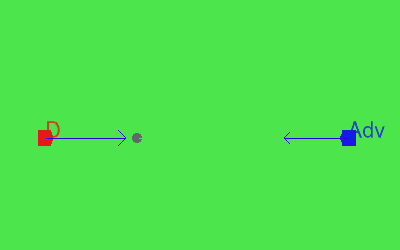
\includegraphics[width = 0.24\textwidth]{dribble1_coupe}
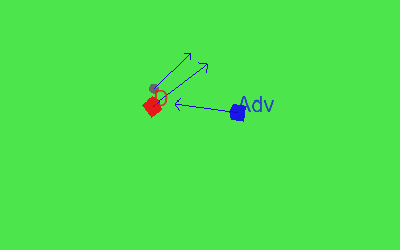
\includegraphics[width = 0.24\textwidth]{dribble2_coupe}
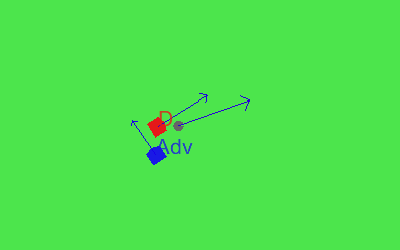
\includegraphics[width = 0.24\textwidth]{dribble3_coupe}
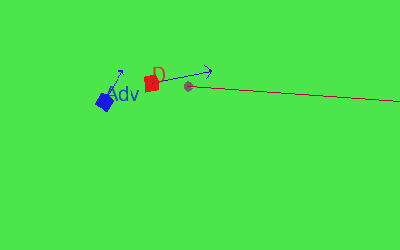
\includegraphics[width = 0.24\textwidth]{dribble4_coupe}
\caption{Exemple de dribble dans un match, Dribbleur en rouge}
\label{Figure5}
\end{figure}

\subsection{Défenseur}

La famille de stratégies de Défenseur a été fondamentale dans les matchs à plusieurs joueurs. Son arbre de décision représentatif est donné sur la Figure \ref{Figure6}. 

\begin{figure}[ht]
\centering
\tikzstyle{block} = [rectangle, rounded corners=3mm, very thick, font=\small, draw=blue!50!white, fill=blue!10!white]
\tikzstyle{decision} = [diamond, rounded corners=3mm, shape aspect=2.5, very thick, font=\small, draw=red!50!white, fill=red!10!white, inner sep=0mm]

\begin{tikzpicture}
\node[decision] (tirer) at (0, 0) {\parbox[c][\height][c]{4cm}{\centering Peut tirer? }};
\node[decision, anchor = north] (tirer_oui) at (-3, -0.6) {\parbox[c][\height][c]{4cm}{\centering Peut faire une passe?}};
\node[decision, anchor = north] (tirer_non) at ( 3, -0.6) {\parbox[c][\height][c]{4cm}{\centering Ballon dans son \\ champ défensif?}};

\draw[thick, -Stealth] (tirer) -- node[midway, above left]{\small Oui} (tirer_oui);
\draw[thick, -Stealth] (tirer) -- node[midway, above right]{\small Non} (tirer_non);

\node[block, anchor = north] (passe_oui) at (-6, -2.5) {\parbox[c][\height][c]{3cm}{\centering Faire la passe}};
\node[decision, anchor = north] (passe_non) at (-3, -3.0) {\parbox[c][\height][c]{4cm}{\centering Il y a un adversaire devant?}};

\draw[thick, -Stealth] (tirer_oui) -- node[midway, above left]{\small Oui} (passe_oui);
\draw[thick, -Stealth] (tirer_oui) -- node[midway, right]{\small Non} (passe_non);

\node[block, anchor = north] (ennemi_oui) at (-5.5, -6.0) {\parbox[c][\height][c]{4cm}{\centering Tirer vers l'avant en évitant l'adversaire}};
\node[block, anchor = north] (ennemi_non) at (-0.5, -6.0) {\parbox[c][\height][c]{4cm}{\centering Tirer vers le centre \\ du but}};

\draw[thick, -Stealth] (passe_non) -- node[midway, above left]{\small Oui} (ennemi_oui);
\draw[thick, -Stealth] (passe_non) -- node[midway, above right]{\small Non} (ennemi_non);

\node[block, anchor = north] (defensif_oui) at (2, -3.5) {\parbox[c][\height][c]{3cm}{\centering Courir vers le ballon}};

\node[block, anchor = north] (defensif_non) at (6, -3.5) {\parbox[c][\height][c]{3cm}{\centering Aller à la position de défense}};

\draw[thick, -Stealth] (tirer_non) -- node[midway, above left]{\small Oui} (defensif_oui);
\draw[thick, -Stealth] (tirer_non) -- node[midway, above right]{\small Non} (defensif_non);
\end{tikzpicture}
\caption{Arbre de décision du Défenseur}
\label{Figure6}
\end{figure}

Notre but était de nous assurer que lorsqu’un attaquant de l’équipe adverse s’attaque à notre Défenseur, ce dernier puisse le confronter et adopter un certain comportement défensif empêchant ainsi aux ennemis de marquer un but. Pour ce faire, nous avons implémenté quelques versions de Défenseur, qui diffèrent essentiellement par leur position de défense et par des simplifications de la branche \og Oui \fg{} du test \og Peut tirer? \fg. Dans un premier moment, nous avons codé une version simplifiée de Défenseur que nous avons appelé Gardien puisque sa position de défense par défaut était le centre de notre but. Dans cette version, lorsqu'il pouvait tirer, il faisait un tir aveugle vers l'avant.

Cette stratégie a bien marché pendant les premières semaines après son implémentation, mais les autres binômes ont réussi à trouver des stratégies d'attaque exploitant des failles de notre gardien, notamment le fait qu'il ne pouvait pas attraper le ballon si sa vitesse était trop élevée. Pour améliorer notre Gardien, nous avons codé une nouvelle version de Défenseur dont la position de défense par défaut n'était pas la cage mais avait un degré de liberté supplémentaire : nous avons choisi une position horizontale \texttt{frac\_p}, représentée comme une fraction de la longueur du champ défensif et passé en argument au Défenseur, de telle sorte que la position de défense avait la position horizontale voulue et était toujours entre le ballon et le centre du but, comme sur la Figure \ref{Figure8}. Notre intention avec cette modification était de faciliter l'interception du ballon. Son but consistait principalement à empêcher le jeu d'attaque de l'équipe adverse.

\begin{figure}[ht]
\centering
\begin{tikzpicture}
\draw (0, -2) -- (0, 2);
\draw[dashed] (-2, -2) node[above left] {\small \texttt{frac\_p}} -- (-2, 2);
\draw[dotted] (-4.2, 2.1) -- (0.2, -0.1);
\fill[black] (-4, 2) circle[radius=0.1];
\node[rectangle, thick, draw=black!50!white, fill=black!30!white, minimum width=0.2cm, minimum height=2cm, anchor = east] (goal) at (0, 0) {};
\node[rectangle, thick, draw=red!80!white, fill=red!30!white, minimum size=0.5cm] at (-2, 1) {};
\end{tikzpicture}
\caption{Position de défense par défaut: position du Dribbleur en rouge, ballon en noir, cage en gris}
\label{Figure8}
\end{figure}

Cette modification de la position de défense a amélioré notre Défenseur mais n'était cependant pas satisfaisante, et nous l'avons modifiée dans la version finale, en augmentant encore un degré de liberté. Pour cela, nous avons choisi un paramètre $\alpha \in [0, 1]$ et défini la position défensive par défaut comme la position sur le segment reliant le ballon au centre de la cage, à une proportion $\alpha$ du centre de la cage et $1 - \alpha$ du ballon. Ainsi, il n'est pas à une position horizontale fixée, mais peut avancer --- même sur le champ d'attaque si le ballon est proche de la cage adverse --- ce qui peut être utile pour récupérer le ballon plus tôt. Remarquons que, si le ballon est trop proche de la cage de défense, il court vers le ballon comme indiqué sur la Figure \ref{Figure6}.

C'est également à ce moment que nous avons codé le mécanisme de passe indiqué sur la Figure \ref{Figure6}. Nous avions auparavant codé une stratégie de passe entre les joueurs, qui prenait en paramètre deux accélérations différentes : une pour tirer et une autre pour faire la passe. L'accélération de passe différente était importante pour que la passe ne soit ni trop longue ni trop courte pour favoriser l’avancement progressif de la balle entre les joueurs jusqu’aux attaquants. 

Pour notre stratégie de passe, lorsque le joueur peut tirer, il calcule la position du joueur qui est le plus proche de lui --- car il est inutile de faire une passe à un joueur qui est loin --- et détermine si ce joueur n'est pas trop proche ni trop loin et si un joueur adversaire n'est pas proche de lui. Une fois la position calculée et les conditions de passe remplies, il fait la passe à ce joueur. Comme nous n'avions pas utilisé cette stratégie de passe de façon isolée, nous l'avons incorporée à notre Défenseur.

Enfin, lorsque le Défenseur a le ballon et ne peut pas faire une passe, plutôt que de tirer aveuglement vers l'avant, il cherche à déterminer si un joueur adverse pourrait intercepter le ballon. Pour ce faire, il détermine les vecteurs entre lui-même et le centre du but adverse et entre lui-même et le joueur adverse le plus proche devant lui, calculant ensuite l'angle entre ces vecteurs. Comme dans le cas du dribble, il choisira, en fonction de la taille de cet angle et de la position de l'adversaire s'il tirera vers le centre du but ou s'il déviera ce tir vers le haut ou le bas.

\subsection{Attaquant}

La stratégie d'Attaquant différemment des autres n'est pas une famille mais une seule stratégie codée spécifiquement pour les matchs 4 contre 4. Nous nous sommes appuyés sur le Défenseur et son arbre de décision représentatif est donné sur la Figure \ref{Figure7}. 

\begin{figure}[ht]
\centering
\tikzstyle{block} = [rectangle, rounded corners=3mm, very thick, font=\small, draw=blue!50!white, fill=blue!10!white]
\tikzstyle{decision} = [diamond, rounded corners=3mm, shape aspect=2.5, very thick, font=\small, draw=red!50!white, fill=red!10!white, inner sep=0mm]

\begin{tikzpicture}
\node[decision] (tirer) at (0, 0) {\parbox[c][\height][c]{4cm}{\centering Peut tirer? }};
\node[decision, anchor = north] (tirer_oui) at (-3, -0.6) {\parbox[c][\height][c]{4cm}{\centering Très proche de la \\ cage adverse?}};
\node[decision, anchor = north] (tirer_non) at ( 3, -0.6) {\parbox[c][\height][c]{4cm}{\centering Il est le plus proche du ballon?}};

\draw[thick, -Stealth] (tirer) -- node[midway, above left]{\small Oui} (tirer_oui);
\draw[thick, -Stealth] (tirer) -- node[midway, above right]{\small Non} (tirer_non);

\node[block, anchor = center] (passe_oui) at (-7, -4.5) {\parbox[c][\height][c]{3cm}{\centering Tirer vers le centre du but}};
\node[decision, anchor = center] (passe_non) at (-1, -4.5) {\parbox[c][\height][c]{4cm}{\centering Il y a un co-équipier plus proche de la cage?}};

\draw[thick, -Stealth] (tirer_oui) -- node[midway, above left]{\small Oui} (passe_oui);
\draw[thick, -Stealth] (tirer_oui) -- node[midway, above right]{\small Non} (passe_non);

\node[decision, anchor = north] (ennemi_oui) at (-3, -6.0) {\parbox[c][\height][c]{4cm}{\centering Peut lui faire une passe?}};

\draw[thick, -Stealth] (passe_non) -- node[midway, above left]{\small Oui} (ennemi_oui);
\draw[thick, -Stealth] (passe_non) -- node[midway, above]{\small Non} (passe_oui);

\node[block, anchor = north] (faire_passe_oui) at (-7, -8.5) {\parbox[c][\height][c]{3cm}{\centering Faire la passe}};

\draw[thick, -Stealth] (ennemi_oui) -- node[midway, above left]{\small Oui} (faire_passe_oui);
\draw[thick, -Stealth] (ennemi_oui) -- node[midway, above right]{\small Non} (passe_oui);

\node[block, anchor = north] (defensif_oui) at (3, -6) {\parbox[c][\height][c]{3cm}{\centering Courir vers le ballon}};

\node[block, anchor = center] (defensif_non) at (5, -4.5) {\parbox[c][\height][c]{3cm}{\centering Aller à la position d'attaque}};

\draw[thick, -Stealth] (tirer_non) -- node[midway, above left]{\small Oui} (defensif_oui);
\draw[thick, -Stealth] (tirer_non) -- node[midway, above right]{\small Non} (defensif_non);
\end{tikzpicture}
\caption{Arbre de décision de l'Attaquant}
\label{Figure7}
\end{figure}

Comme pour le Défenseur, l'Attaquant a une position par défaut s'il ne peut pas tirer, même si le test pour qu'il aille vers cette position n'est pas la même. Cette position est aussi définie par un paramètre de pondération $\alpha$ et se situe dans le segment reliant le ballon et le centre de la cage adverse. Il court vers le ballon seulement s'il est le joueur le plus proche parmi tous (y compris les joueurs adverses). Lorsqu'il a le ballon, il décide entre tirer vers le centre du but ou faire une passe, d'après les positions de ses co-équipiers, avec le même mécanisme de passe du Défenseur.

Cette stratégie a été fondamentale pour avoir des résultats satisfaisants dans les matchs à 4 joueurs. En effet, avant de la coder, notre équipe avait des difficultés pour marquer des buts car toutes nos stratégies non défensives avaient comme comportement par défaut de courir vers le ballon si elles n'en avaient pas possession. Par conséquent, tous les joueurs couraient vers le ballon et, si l'équipe en récupérait la possession, l'attaque était difficile à cause du mauvais positionnement des joueurs. Dans un premier moment nous avons cru que l'optimisation par l'algorithme génétique de 4 joueurs (2 Dribbleurs et 2 Défenseurs) serait suffisante pour régler ce problème, ce qui n'a pas été le cas, nous motivant donc à créer cette nouvelle stratégie.

\section{Optimisation des stratégies}
\label{4}

Les familles de stratégies décrites dans la Section \ref{3} ont été créées toutes avec des paramètres passés en argument au constructeur de la \texttt{Strategy} correspondante, pour faciliter leur optimisation. Si dans un premier moment cette optimisation était faite à la main cela est devenu vite impraticable avec l'énorme quantité de paramètres. Dans cette section nous présenterons les 3 techniques d'optimisation utilisés dans ce projet : Les 2 techniques de recherche de paramètres optimaux --- recherche exhaustive et recherche par l'algorithme génétique --- et la création automatique des arbres de décision, comme celles de la section précédente, à partir des stratégies très simples.  

\subsection{Recherche exhaustive}

La recherche exhaustive d'un optimum consiste à tester toutes les possibilités des paramètres afin de voir quelle est la meilleure combinaison entre elles. Pour ce faire les paramètres continus doivent être discrétisés pour avoir une quantité finie de cas à tester. Cette recherche a une complexité exponentielle par rapport à la quantité de paramètres car il faut chercher sur le produit cartésien des intervalles de valeurs de chaque paramètre. Ainsi pour $n$ paramètres chacun avec $m$ valeurs possibles, nous avons une complexité de $m^n$ cas à tester. 

Le premier moment où nous avons eu besoin de l'optimisation dans ce projet a été lors du chalenge consistant à faire le nombre maximal de buts en 10000 pas de temps (sans joueur adverse). Pour ce chalenge nous avons utilisé le Fonceur de la Section \ref{3} sans prévision de la position du ballon et accélération de course maximale et comme seule variable d'optimisation l'accélération de tir. Cette optimisation a été faite par une recherche exhaustive en discrétisant l’intervalle d'accélérations possibles et cherchant à minimiser le temps nécessaire pour marquer 10 buts. Comme celle-ci a été fait avant la partie du cours sur la recherche exhaustive, nous avons dû coder par nous-mêmes tous les fonctions nécessaires. Le résultat de cette optimisation est présenté dans la Figure \ref{Figure2}. 

\begin{figure}[ht]
\centering
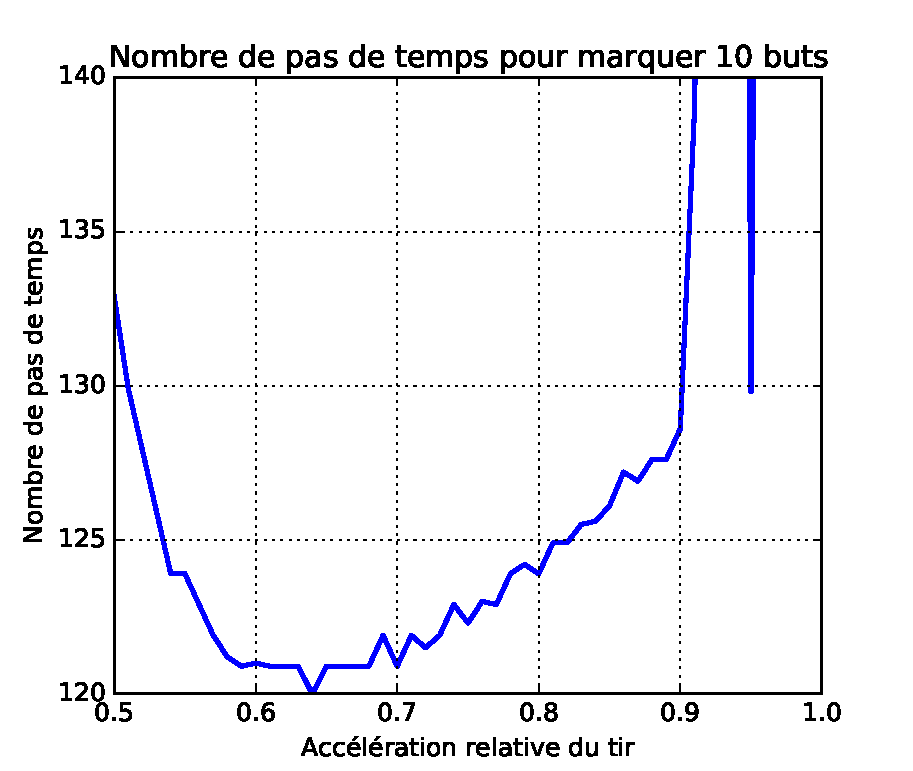
\includegraphics[scale = 0.67]{param_search_chalenge}
\caption{Recherche exhaustive de l'accélération de tir optimale}
\label{Figure2}
\end{figure}

L'accélération est donné en fraction de l'accélération maximale d'un tir. Nous pouvons voir sur la figure que sa valeur optimale est 0.64. En réalisant de simulations nous avons pu constater que, avec cette accélération, 2 tirs sont nécessaires pour marquer un but. Nous avons donc codé une recherche exhaustive sur 2 paramètres (correspondant chacun à l’accélération d'un tir) mais le résultat était que 2 tirs de la même intensité étaient l'optimum. Par contre, l' accélération optimale pour ce challenge n'est pas bonne pour les matchs.

Cette technique n'est pas adaptée pour la plupart des optimisations que nous avons dû faire dans ce projet car nous avions une dizaine de paramètres environ par stratégie et la complexité exponentielle rendait cela impraticable. Nous nous sommes alors appuyés sur des méthodes plus adaptées à cette quantité de paramètres.

\subsection{Algorithme génétique}

La recherche génétique est, comme la recherche exhaustive, une méthode pour trouver un optimum sur un ensemble donné de paramètres, mais, différemment de celle-ci, on ne teste pas toutes les combinaisons possibles de paramètres afin d'avoir une recherche dans un temps raisonnable, ce qui conduit à un optimum approché.

Nous avons implémenté l'algorithme génétique de la façon suivante : on commence par choisir une taille de population \texttt{nb\_players}, chaque \emph{individu} de cette population étant un vecteur de paramètres choisi initialement de façon aléatoire en respectant les intervalles de valeurs de chaque paramètre. Même s'il n'est pas nécessaire de discrétiser les paramètres continus, nous avons choisi de le faire dans ce projet après avoir remarqué que des petites variations de paramètres ne changent pas le comportement d'un joueur. Une fois les individus choisis, il faut, pour chaque individu, tester le critère à optimiser. Dans notre implémentation, nous avons cherché à optimiser le nombre de points obtenus au total après un nombre donné de matchs \texttt{trials} contre chacune des équipes adverses codées par les autres binômes. Un match gagné donne 3 points, un match nul donne 1 point, et un match perdu ne donne pas de points. Nous avons ainsi un score pour chaque individu.

Une fois le score de tous les individus calculé, nous créons une nouvelle génération d'individus. Un pourcentage \texttt{pourcent\_meilleurs} de cette génération correspond aux individus de la génération précédente ayant eu les plus grands scores. Parmi les individus restants, on garde dans la nouvelle génération un pourcentage \texttt{pourcent\_autres} afin de garder une diversité de paramètres dans la population et essayer d'éviter la convergence vers un optimum local. La somme des pourcentages \texttt{pourcent\_meilleurs} et \texttt{pourcent\_autres} doit être inférieure à $100 \%$, et les individus restants seront créé par reproduction des individus déjà choisis. Pour la reproduction, on choisit de façon aléatoire deux individus, appelés \emph{parents}. Ensuite, chaque paramètre du nouvel individu est choisi parmi les paramètres correspondants de ses deux parents de façon aléatoire. On implémente également la possibilité d'avoir une \emph{mutation}, c'est-à-dire que le paramètre soit une valeur aléatoire plutôt qu'une copie de la valeur d'un parent, cette mutation ayant lieu avec une probabilité de \texttt{proba\_mut} pour chaque paramètre.

Le calcul du score est refait avec cette nouvelle population, et on répète cette procédure un nombre donné \texttt{nb\_generations} de fois. À la fin, on choisi l'individu avec le meilleur score de la dernière population. Ses paramètres sont ainsi ceux qui seront utilisés dans le tournoi. Il est à noter qu'un individu de notre population est un vecteur contenant les paramètres de \emph{tous} les joueurs de l'équipe, le calcul du score étant donc différent selon le nombre de joueurs car, bien sûr, le nombre de paramètres augmente avec la quantité de joueurs. Nous avons choisi d'avoir un seul vecteur avec les paramètres de tous les joueurs pour optimiser l'ensemble de l'équipe plutôt que des joueurs individuellement.

Depuis que l'algorithme génétique a été codé, nous l'avons utilisé systématiquement à chaque semaine pour améliorer nos équipes. Bien que son temps d'exécution soit long, il a été essentiel pour nos bons résultats, car il permettait d'adapter nos stratégies à celles des autres binômes. Cette optimisation, bien que nécessaire, n'était pas suffisante à chaque semaine pour avoir un bon rang, et a été accompagnée par des améliorations des stratégies jusqu'à ce qu'elles arrivent aux formes finales présentées dans la Section \ref{3}. Il est aussi intéressant à noter que, dans les matchs 4 contre 4, même si nous avons mis 2 Défenseurs, l'algorithme génétique a choisi des paramètres assez diverses pour eux, ce qui a donné des joueurs différents et complémentaires avec la même stratégie de base.

Pour illustrer le fonctionnement de l'algorithme génétique, nous représentons dans la Figure \ref{Figure9} l'évolution du score moyen des individus et de leurs diversités moyennes en fonction de l'indice de la génération. La diversité d'un paramètre a été calculée comme le nombre de valeurs différentes que ce paramètre prend sur la génération donnée, et la diversité moyenne correspond à la moyenne des diversités de tous les paramètres dans cette génération. Cette figure correspond à une simulation de matchs 4 contre 4, pour lesquels nous avons 29 paramètres. Elle a été réalisée pour le tournoi de la semaine 10, le premier à avoir des matchs 4 contre 4 et utilise une population de 20 individus, avec 5 matchs contre chaque équipe et 11 générations, ce qui a pris un temps de calcul de 26h.

\begin{figure}[ht]
\centering
\begin{tabular}{@{} >{\centering} m{0.5\textwidth} @{} >{\centering} m{0.5\textwidth} @{}}
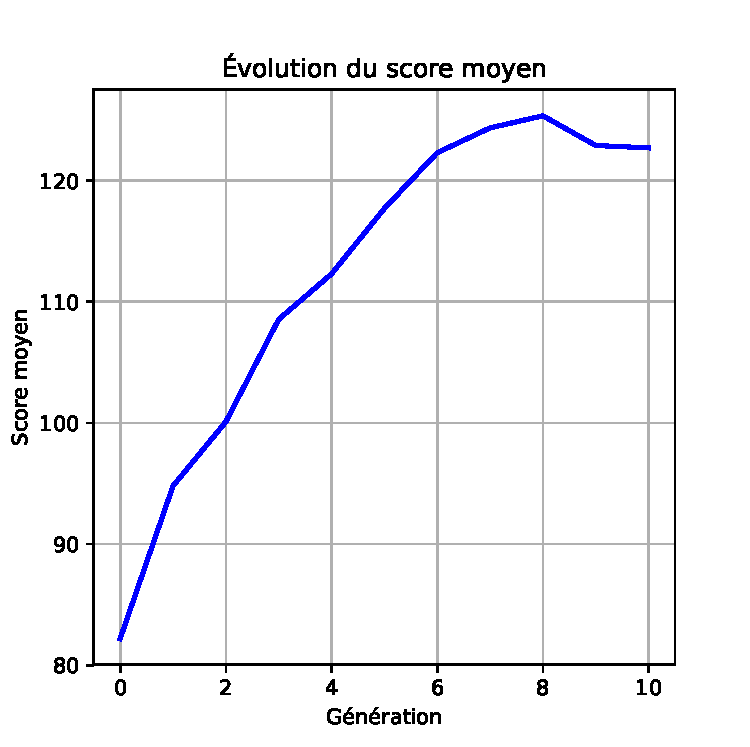
\includegraphics[width=0.5\textwidth]{score_moyen} & 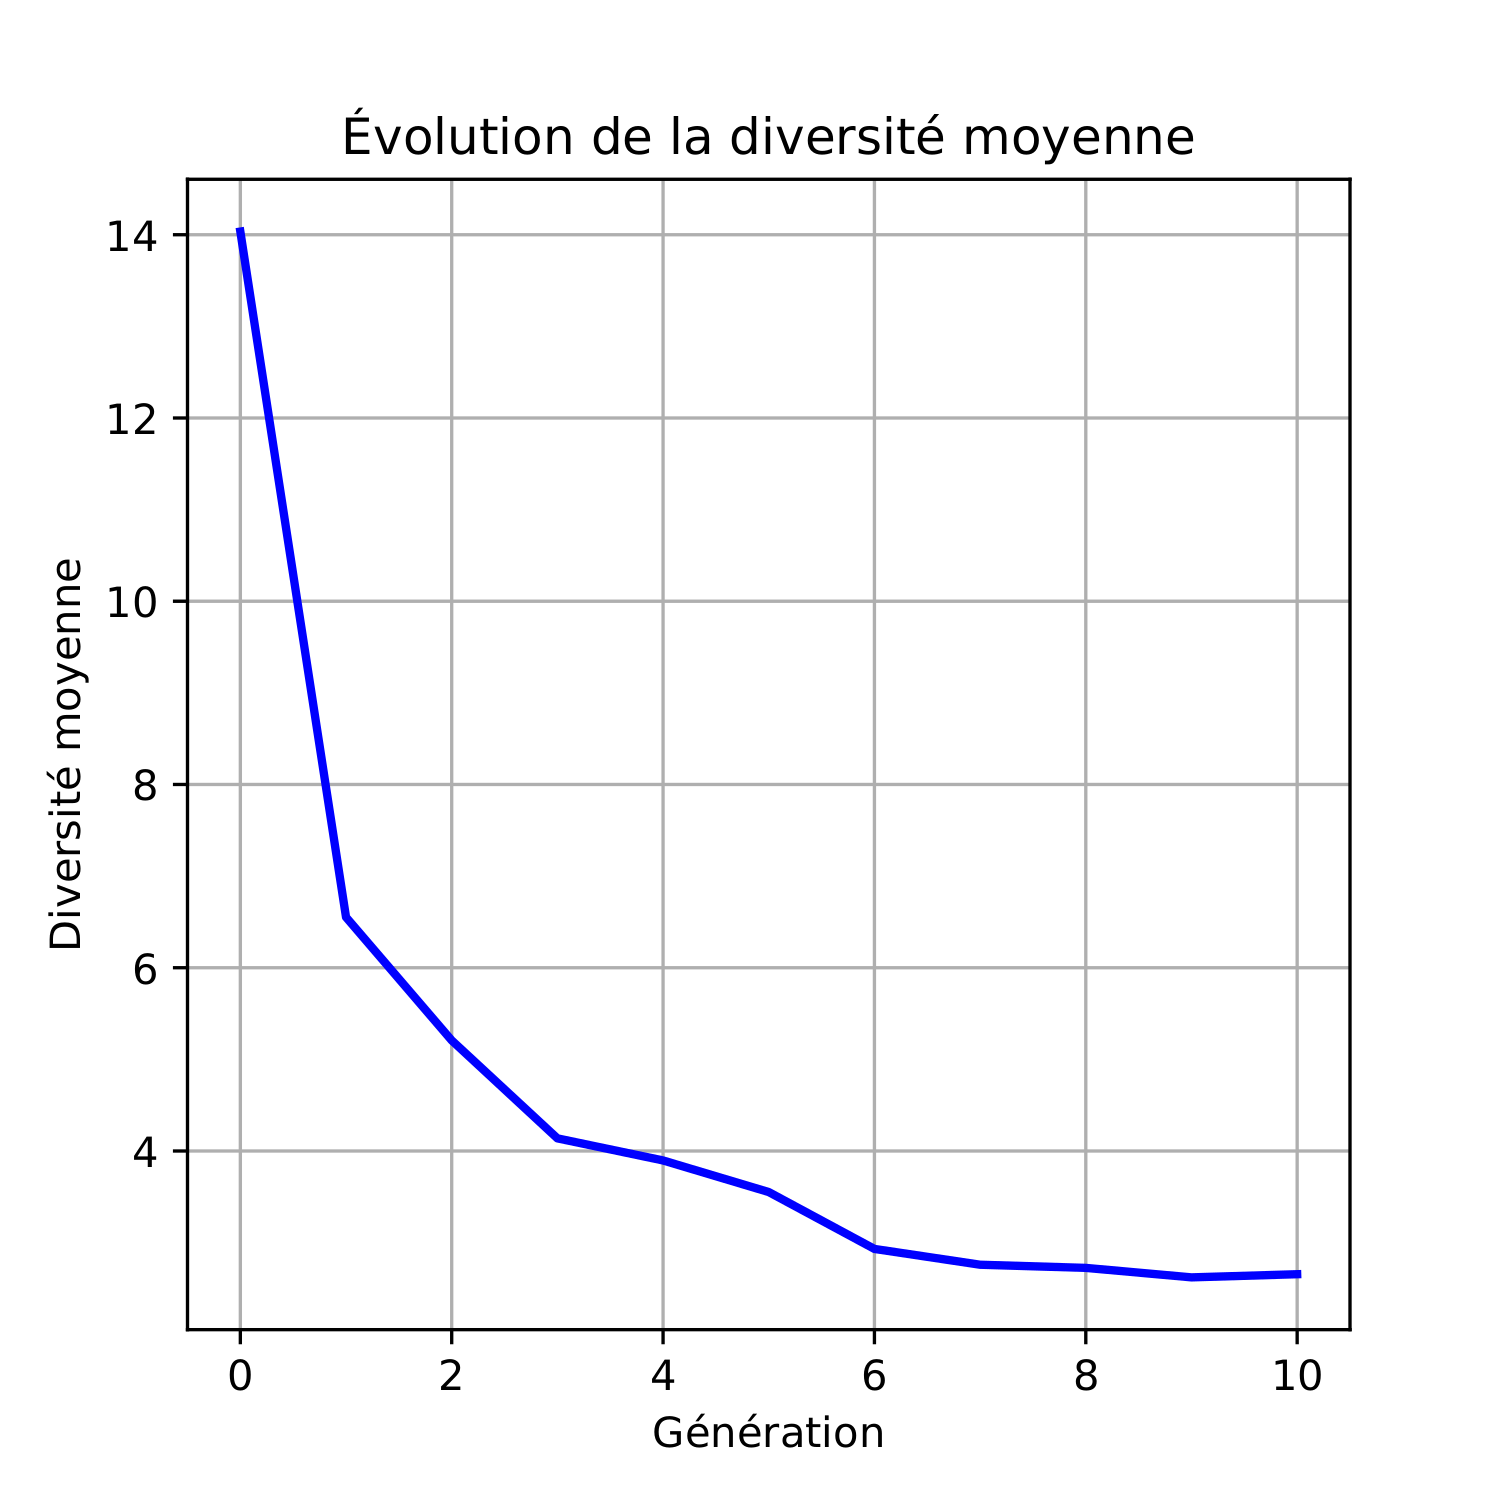
\includegraphics[width=0.5\textwidth]{diversite_moyenne} \tabularnewline
(a) & (b) \tabularnewline
\end{tabular}
\caption{Évolution en fonction des générations (a) du score moyen et (b) de la diversité moyenne}
\label{Figure9}
\end{figure}

On remarque sur la Figure \ref{Figure9}(a) la croissance du score moyen, comme attendu. Pour cette simulation, avec 9 autres binômes et 5 matchs par binôme, la quantité maximale de points possible est de 135, ce qui montre que les résultats obtenus sont très satisfaisants, avec un nombre moyen de points de 122,7 et un nombre maximal de 133. Remarquons que 133 points correspond à 44 victoires et un match nul, sans défaites. Ce sont les paramètres correspondants au score de 133 points qui ont été utilisés pour la semaine 10, ce qui est cohérent avec notre classement cette semaine.

La Figure \ref{Figure9}(b) montre que la diversité moyenne décroit avec le nombre de générations. Ainsi, comme espéré, les individus convergent vers une situation où plusieurs joueurs partagent les mêmes valeurs de paramètres. Il est à noter que, comme on a une population de 20 individus, la diversité est nécessairement inférieure ou égale à 20. Cependant, certains paramètres sont discrétisés en moins de 20 valeurs possibles, ce qui explique la diversité d'environ 14 pour la première génération.

\subsection{Arbres de décision}

Différemment de l'optimisation par recherche exhaustive ou par l'algorithme génétique, l'optimisation par arbre de décision ne cherche pas à trouver les meilleurs paramètres pour une stratégie ou une équipe donnée, mais plutôt à construire de façon intelligente, à partir du comportement attendu des joueurs, un arbre de décision, similaire à ceux des Figures \ref{Figure1}, \ref{Figure3}, \ref{Figure6} et \ref{Figure7}. Pour cela, il faut d'abord coder des stratégies simples, correspondant essentiellement aux blocs en bleu des arbres représentés précédemment. Pour notre implémentation, nous avons codé 6 stratégies élémentaires : fonceur, gardien, défenseur, dribbleur, passe et attaquant. L'enjeu est de choisir automatiquement les blocs de décision, c'est-à-dire les blocs en rouge des arbres précédents.

L'objectif est, à la fin, d'avoir une fonction qui, étant donné un état du jeu du type \texttt{SoccerState}, renvoie l'une des 6 stratégies, celle la plus adaptée pour cet état. Comme un \texttt{SoccerState} contient trop d'informations, nous avons choisi des caractéristiques, ou \emph{features}, qui seront les données prises en compte par cette fonction. Nous avons sélectionné 9 caractéristiques pour les matchs 1 contre 1 et 13 pour les matchs 2 contre 2, comprenant, par exemple, la distance du joueur au ballon, la distance du ballon à la cage adverse, ou encore des booléens comme l'existence d'un gardien adversaire.

L'apprentissage par arbre de décision est une méthode dite supervisée, c'est-à-dire qu'il faut lui fournir un ensemble très grand de données comportant un couple composée de valeurs pour les features et la stratégie à choisir pour ces valeurs. Il faut donc avoir deux étapes : une première pour créer ces couples features--stratégies et une deuxième pour apprendre l'arbre à partir de ces données. Le code pour la deuxième étape a été fourni, il s'agit d'un code se basant sur la bibliothèque \texttt{sklearn} de Python et ses fonctions spécifiques pour les arbres de décision disponibles dans \texttt{sklearn.tree}.

Pour la première étape, nous avons utilisé deux méthodes. La première, basée sur le code fourni, consiste à \og jouer \fg. Plus précisément, le code fourni présentait un moyen d'associer, à chaque stratégie élémentaire, une touche du clavier, et de lancer une simulation où l'on peut alterner entre ces stratégies à l'aide de ces touches. À chaque fois que l'on appuie sur une touche, on enregistre les valeurs des features et la stratégie choisie pour ces valeurs. Nous avons modifié le code fourni, pour permettre par exemple de charger un fichier avec des couples features--stratégies déjà enregistrés et y ajouter des nouveaux couples obtenus par une nouvelle simulation, afin d'enregistrer que les couples correspondants aux matchs gagnés. Une mini-interface utilisant le terminal a été également mise en place pour faciliter les simulations, permettant par exemple de choisir facilement contre quelle stratégie jouer.

La deuxième méthode utilisée pour construire des couples features--stratégies con\-siste à créer un état au hasard et demander sur le terminal quelles stratégies doivent être choisies pour cet état, enregistrant ensuite le couple features--stratégie correspondant. Cette implémentation a été utilisée uniquement pour les matchs 2 contre 2, où l'on enregistre les couples séparément pour les deux joueurs. En effet, pour les matchs 2 contre 2, la méthode de lancer une simulation est plus difficile à utiliser car il faut contrôler deux joueurs en même temps.

Un exemple d'arbre de décision crée par notre code est donné sur la Figure \ref{Figure10}. Il s'agit d'un petit arbre, entrainé avec uniquement 74 couples features--stratégies, présenté ici car les arbres avec des centaines de couples deviennent illisibles.

\begin{figure}[ht]
\centering
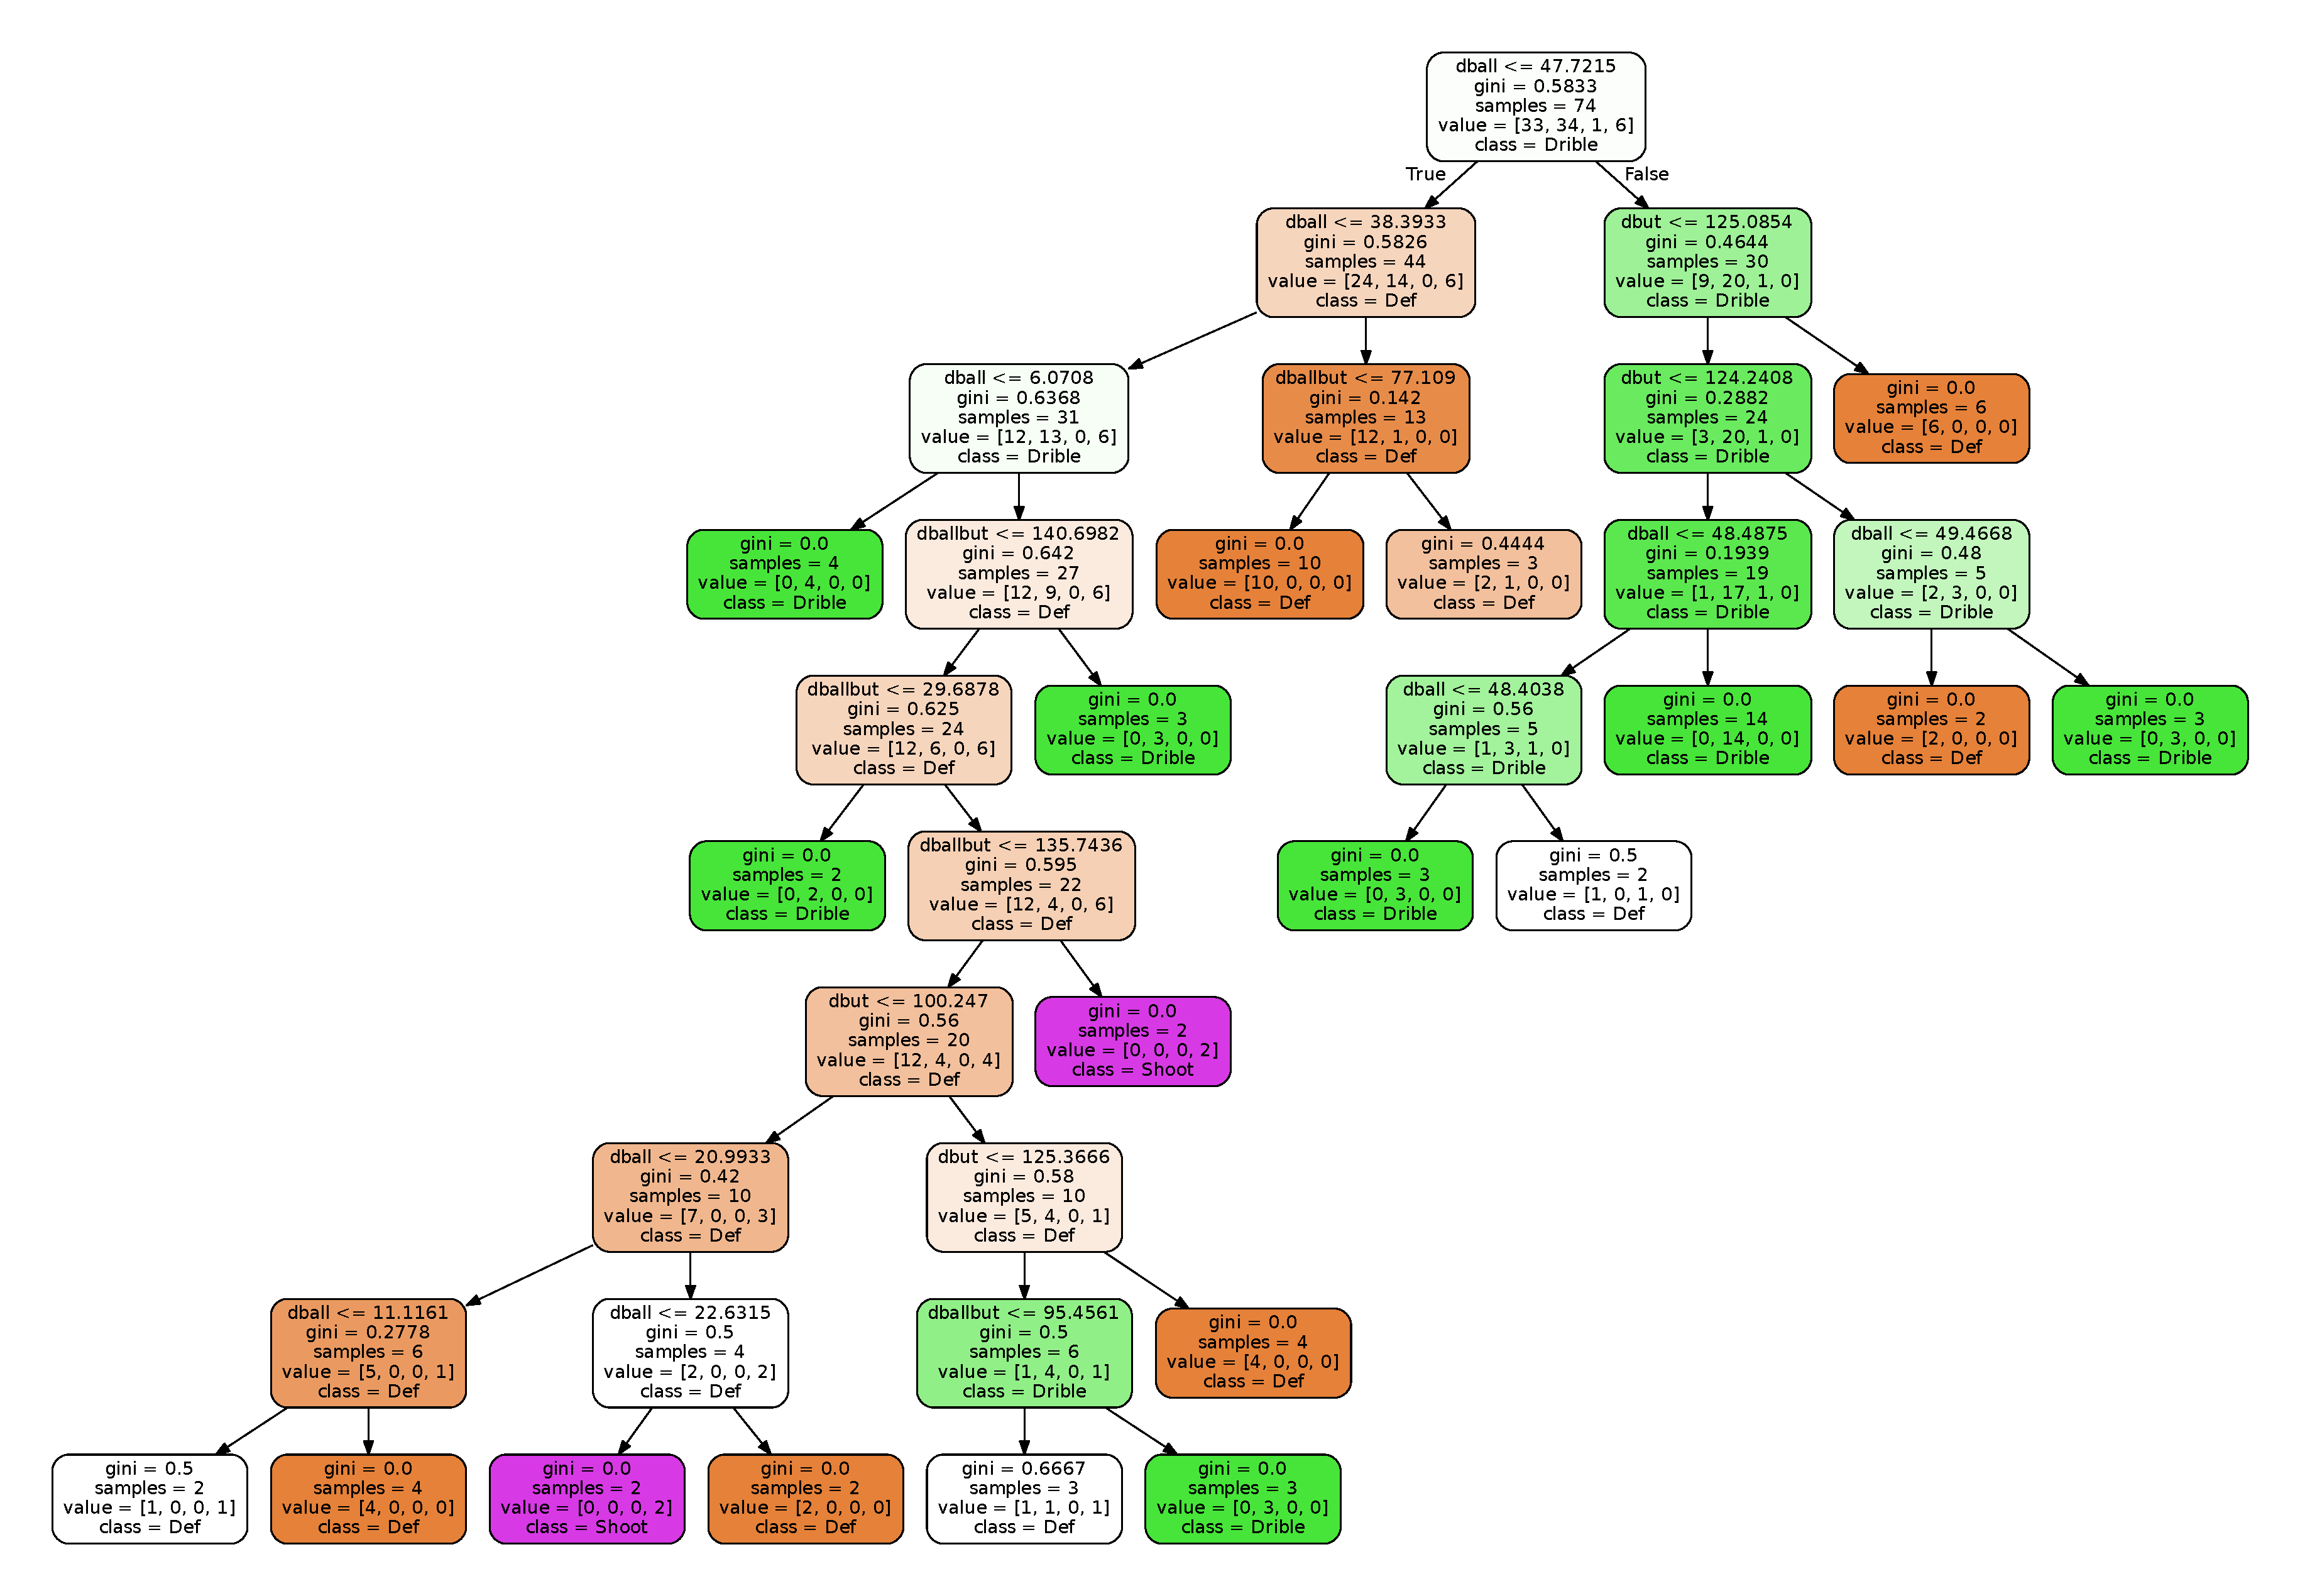
\includegraphics[width=\textwidth]{test_arbre}
\caption{Exemple d'arbre de décision}
\label{Figure10}
\end{figure}

Pour les matchs en 1 contre 1, les arbres de décision obtenus avec notre code marchait de façon satisfaisante quand elles étaient entrainées contre une même stratégie adverse. Par contre, en essayant de coder un même arbre en jouant contre des stratégies de plusieurs binômes, nous n'avons pas obtenu de bons résultats, même après avoir fourni environ 500 couples features--stratégies pour l'entrainement de l'arbre. Cela peut être expliqué par deux difficultés que nous avons rencontrées. D'une part, les stratégies des autres binômes étaient assez différentes entre elles, ce que veut dire que nos choix de stratégies élémentaires pour chaque ensemble de features était assez diverse. Cela a conduit à un joueur qui, à la fin, était optimisé contre une sorte de \og stratégie moyenne \fg{} des autres binômes, mais sans être particulièrement effectif contre aucune stratégie adverse. D'autre part, nous avons constaté que, dans certaines situations, le choix de la bonne stratégie n'était pas évident et pourrait changer si l'état était légèrement différent. Pour avoir un arbre capable de trancher correctement, il faudrait probablement avoir beaucoup plus de couples features--stratégies. Or, ces couples étant crées à la main en jouant à des matchs, en créer plusieurs milliers prend un temps inenvisageable. Il faut cependant noter que le joueur par arbre de décision créé était plutôt bien performant en défense, mais, une fois qu'il récupérait le ballon, il le perdait en attaque systématiquement sans être capable de faire un but.

Pour les matchs en 2 contre 2, nous avions la difficulté supplémentaire de devoir jouer avec deux joueurs en même temps pour créer les couples features--stratégies des deux joueurs. Cela a conduit à plusieurs matchs où nos choix nous conduisaient à la défaite. Or, un arbre de décision ne pourra pas jouer beaucoup mieux que la personne qui lui a fourni les données. D'autre part, la difficulté avec la deuxième méthode pour construire des couples features--stratégies était que, avec uniquement une image de l'état et sans voir l'évolution du jeu, il était difficile de choisir la stratégie optimale pour cet état.

À cause de ces difficultés, nous avons priorisé l'optimisation par l'algorithme génétique. Bien que cette méthode ne permette pas d'aller au-delà des structures simples d'arbres de décision de la Section \ref{3}, l'optimisation des paramètres nous a permis en pratique d'avoir des joueurs plus performants que nous-même lors de la création à la main des couples features--stratégies pour l'arbre de décision.

\section{Conclusion}

Ce projet a été l'occasion, d'une part, de s’entraîner à la programmation orientée objet en Python, en réfléchissant à un problème pour proposer des algorithmes qui le résolvent. Nous avons pratiqué la réflexion en binôme et le travail en équipe, en décomposant notre problème en tâches plus simples et les partageant. L'évolution de notre code nous a permis de comprendre des difficultés du projet en soi, comme les questions d'organisation générale du code ou les difficultés inhérentes au jeu SoccerSimulator et à la compétition hebdomadaire entre binômes.

D'autre part, ce projet nous a également permis de connaitre des méthodes importantes en intelligence artificielle et optimisation, comme l'algorithme génétique, qui permet le choix des paramètres quasi-optimaux sans supervision, et les arbres de décision, qui ont l'avantage de ne pas avoir besoin d'une structure pré-définie avec paramètres mais nécessitent un apprentissage supervisée avec une très grande quantité de données. Le contact avec les méthodes précédentes nous donne envie d'approfondir nos connaissances sur ce domaine.

\end{document}
